% -*- mode: noweb; noweb-default-code-mode: R-mode; -*-
%\VignetteIndexEntry{FAQ and design desicions}

\documentclass[a4paper]{article}

\usepackage{ucs}
\usepackage[utf8x]{inputenc}
\usepackage[T1]{fontenc}
\usepackage[sort&compress]{natbib}
\usepackage{hyperref}
\usepackage{graphics}
\usepackage{float}
\floatplacement{figure}{htbp}
\floatstyle{ruled}
\restylefloat{figure}
\renewcommand{\floatpagefraction}{0.8}

\author{Jari Oksanen}
\title{Frequently Asked Questions}

\usepackage{/usr/local/lib/R/share/texmf/Sweave}
\begin{document}


\maketitle

\begin{abstract}

\noindent
The document answers some frequently asked questions and explains some
design decisions I have made in vegan.

\end{abstract}

\tableofcontents

\section{Scaling in redundancy analysis}

This chapter discusses the scaling of scores (results) in redundancy
analysis and principal component analysis performed by function
\texttt{rda} in the \texttt{vegan} library.  Principal component
analysis, and hence redundancy analysis, is a variant of singular
value decomposition (\textsc{svd}).  Functions \texttt{rda} and
\texttt{prcomp} (library \texttt{mva}) even use \textsc{svd}
internally in their algorithm.  In \textsc{svd} a centred data matrix
is decomposed into orthogonal components so that $x_{ij} = \sum_k
\sigma_k u_{ik} v_{jk}$, where $u_{ik}$ and $v_{jk}$ are orthonormal
coefficient matrices and $\sigma_k$ are singular values.
Orthonormality means that sum of squared columns is one and their
cross-product is zero, or $\sum_i u_{ik}^2 = \sum_j v_{jk}^2 = 1$, and
$\sum_i u_{ik} u_{il} = \sum_j v_{jk} v_{jl} = 0$ for $k \neq l$. This
is a decomposition, and the original matrix is found exactly from the
singular vectors and corresponding singular values, and first two
singular components give the best rank $=2$ least squares estimate of
the original matrix.

Principal component analysis is often presented (and performed in
legacy software) as an eigenanalysis of covariance matrices.  Instead
of data matrix, we analyse a matrix of covariances and variances
$\mathbf{S}$.  The result will be orthonormal coefficient matrix
$\mathbf{U}$ and eigenvalues $\mathbf{\Lambda}$.  The coefficients
$u_{ik}$ ares identical to \textsc{svd} (except for possible sign
changes), and eigenvalues $\lambda_k$ are related to the corresponding
singular values by $\lambda_k = \sigma_k^2 /(n-1)$.  With classical
definitions, the sum of all eigenvalues equals the sum of variances of
species, or $\sum_k \lambda_k = \sum_j s_j^2$, and it is often said
that first axes explain a certain maximized proportion of total
variance in the data.  The other orthonormal matrix $\mathbf{V}$ can
be found indirectly as well, so that we have the same components in
both methods.

The coefficients $u_{ik}$ and $v_{jk}$ are of the same (unit) length
for all axes $k$, but singular values $\sigma_k$ or eigenvalues
$\lambda_k$ give the information of the importance of axes, or the
`axis lengths.'  Instead of the orthonormal coefficients, or equal
length axes, it is customary to use eigenvalues to scale at least one
of the alternative scores to reflect the importance of axes or
describe the true configuration of points.  Table \ref{tab:scales}
shows some alternative scalings used in various software.  These
alternatives apply to principal components analysis in all cases, and
in redundancy analysis, they apply to species scores and constraints or
linear combination scores; weighted averaging scores have somewhat
wider dispersion.

\begin{table}
  \caption{\label{tab:scales} Alternative scalings for \textsc{rda} used
    in the functions \texttt{prcomp} and \texttt{princomp} (package
    \texttt{mva}), and the one used in the \texttt{vegan} function \texttt{rda}
    and the proprietary software \texttt{Canoco}
    scores in terms of orthonormal species ($u_{ik}$) and site scores
    ($v_{jk}$), eigenvalues ($\lambda_k$), number of sites  ($n$) and
    species standard deviations ($s_j$). In \texttt{rda},
    $\mathrm{const} = \sqrt[4]{(n-1) \sum \lambda_k}$.  Corresponding
    negative scaling in \texttt{vegan}
    and corresponding positive scaling in \texttt{Canoco} is derived
    dividing each  species by its standard deviation $s_j$ (possibly
    with some additional constant multiplier).  }
\begin{tabular}{lcc}
& \textbf{Site scores} $u_{ik}^*$ &
\textbf{Species scores} $v_{jk}^*$ \\
\texttt{prcomp, princomp} &
$u_{ik} \sqrt{n-1} \sqrt{\lambda_k}$ &
$v_{jk}$ \\
\texttt{rda, scaling=1} &
$u_{ik} \sqrt{\lambda_k/ \sum \lambda_k} \times \mathrm{const}$ &
$v_{jk} \times \mathrm{const}$
\\
\texttt{rda, scaling=2} &
$u_{ik} \times \mathrm{const}$ &
$v_{jk} \sqrt{\lambda_k/ \sum \lambda_k} \times \mathrm{const}$  \\
\texttt{rda, scaling=3} &
$u_{ik} \sqrt[4]{\lambda_k/ \sum \lambda_k} \times \mathrm{const}$ &
$v_{jk} \sqrt[4]{\lambda_k/ \sum \lambda_k} \times \mathrm{const}$ \\
\texttt{rda, scaling < 0} &
$u_{ik}^*$ &
$\sqrt{\sum \lambda_k /(n-1)} s_j^{-1} v_{jk}^*$
\\
\texttt{Canoco, scaling=-1} &
$u_{ik} \sqrt{n} \sqrt{\lambda_k / \sum \lambda_k}$ &
$v_{jk} \sqrt{n}$ \\
\texttt{Canoco, scaling=-2} &
$u_{ik} \sqrt{n}$ &
$v_{jk} \sqrt{n} \sqrt{\lambda_k / \sum \lambda_k}$
\\
\texttt{Canoco, scaling=-3} &
$u_{ik} \sqrt{n} \sqrt[4]{\lambda_k / \sum \lambda_k}$ &
$v_{jk} \sqrt{n} \sqrt[4]{\lambda_k / \sum \lambda_k}$
\end{tabular}
\end{table}

In community ecology, it is common to plot both species and sites in
the same graph.  If this graph is a graphical display of \textsc{svd},
or a graphical, low-dimensional approximation of the data, the graph
is called a biplot.  The graph is a biplot if the transformed scores
satisfy $x_{ij} = c \sum_k u_{ij}^* v_{jk}^*$ where $c$ is a scaling
constant.  In functions \texttt{princomp}, \texttt{prcomp} and
\texttt{rda}, $c=1$ or the plotting scores are the straight biplot
scores so that the singular values (or eigenvalues) are expressed for
sites, and species are left unscaled.  For \texttt{Canoco} $c = n^{-1}
\sqrt{n-1} \sqrt{\sum \lambda_k}$ with positive \texttt{Canoco}
scaling values. All these $c$ are constants for a matrix, so these are
all biplots with different internal scaling of species and site scores
with respect to each other.  For \texttt{Canoco} with postive scaling
values and \texttt{vegan} with negative scaling values, no constant
$c$ can be found, but the correction is dependent on species standard
deviations $s_j$, so this alternative does not define a biplot.

There is no natural way of scaling species and site scores to each
other, but all functions and programs above selected different
strategies.  The eigenvalues in redundancy and principal components
analysis are scale dependent and change when the the data are
multiplied by a constant.  If we have percent cover data, the
eigenvalues are typically very high, and the scores scaled by
eigenvalues will have much wider dispersion than the orthonormal set.
If we express the percentages as proportions, or divide the matrix by
$100$, the eigenvalues will be reduced by factor $100^2$, and the
scores scaled by eigenvalues will have much narrower dispersion than
the orthonormal set.  For graphical biplots we should be able to fix
the relation and make it invariant for scale changes.  The solution
adoption in the R standard function \texttt{biplot.princomp} is to
scale site and species scores independently, and typically very
differently, but plot each with separate scales so that both sets fill
the graph area.  The solution in \texttt{Canoco} and \texttt{rda} is
to use proportional eigenvalues $\lambda_k / \sum \lambda_k$ instead
of original eigenvalues.  These proportions are invariant with scale
changes, and typically they have a nice range for plotting two data
sets in the same graph.

In this chapter, I used always centred data matrices.  In principle
\textsc{svd} could be done with original, non-centred data, but
there is no option for this in \texttt{rda}, because I think that
non-centred analysis is dubious and I do not want to encourage its use
(if you think you need it, you are certainly so good in programming
that you can change that one line in \texttt{rda.default}).  I do
think that the arguments for non-centred analysis are often twisted,
and the method is not very good for its intended purpose, but there
are better methods for finding fuzzy classes.  Normal, centred
analysis moves the origin to the average of all species, and the
dimensions describe differences from this average.  Non-centred
analysis leaves the origin in the empty site with no species, and the
first axis usually runs from the empty site to the average
site. Second and third non-centred components are often very similar
to first and second (etc.) centred components, and the best way to use
non-centred analysis is to discard the first component and use only
the rest. This is better done with directly centred analysis.


\section{Why to use weighted averages scores instead of linear
  combinations in constrained ordination}

Constrained ordination methods such as Constrained Correspondence
Analysis (CCA) and Redundancy Analysis (RDA) produce two kind of site
scores \cite{Braak86, Palmer93}:
\begin{itemize}
\item
LC or Linear Combination Scores which are linear combinations of
constraining variables.
\item
WA or Weighted Averages Scores which are such weighted averages of
species scores that are as similar to LC scores as possible.
\end{itemize}
Many computer programs for constrained ordinations give only or
primarily LC scores, following Mike Palmer's recommendation
\cite{Palmer93}.  However, functions \texttt{cca} and \texttt{rda} in
the \texttt{vegan} package use primarily WA scores. This chapter
explains the reasons for this choice.

Briefly, the main reasons are that
\begin{itemize}
\item
LC scores \emph{are} linear combinations, so they give us only the
(scaled) environmental variables. This means that they are
independent of vegetation and cannot be found from the species
composition.  Moreover, identical combinations of environmental
variables give identical LC scores irrespective of vegetation.
\item
Bruce McCune has demonstrated that noisy environmental variables
result in deteriorated LC scores whereas WA scores tolerate some errors
in environmental variables \cite{McCune97}.  All environmental
measurements contain some errors, and therefore it is safer to use WA
scores.
\end{itemize}
This articles studies mainly the first point.  The users of
\texttt{vegan} have a choice of either LC or WA (default) scores, but
after reading this article, I believe that most of them do not want to
use LC scores, because they are not what they were looking for in
ordination.

\subsection{LC Scores are Linear Combinations}

Let us perform a simple CCA analysis using only two environmental
variables so that we can see the constrained solution completely in
two dimensions:
\begin{Schunk}
\begin{Sinput}
> library(vegan)
> data(varespec)
> data(varechem)
> orig <- cca(varespec ~ Al + K, varechem)
\end{Sinput}
\end{Schunk}
Function \texttt{cca} in \texttt{vegan} uses WA scores as
default. So we must specifically ask for LC scores
(Fig. \ref{fig:ccalc}).
\begin{figure}
\begin{center}
\begin{Schunk}
\begin{Sinput}
> plot(orig, dis = c("lc", "bp"))
\end{Sinput}
\end{Schunk}
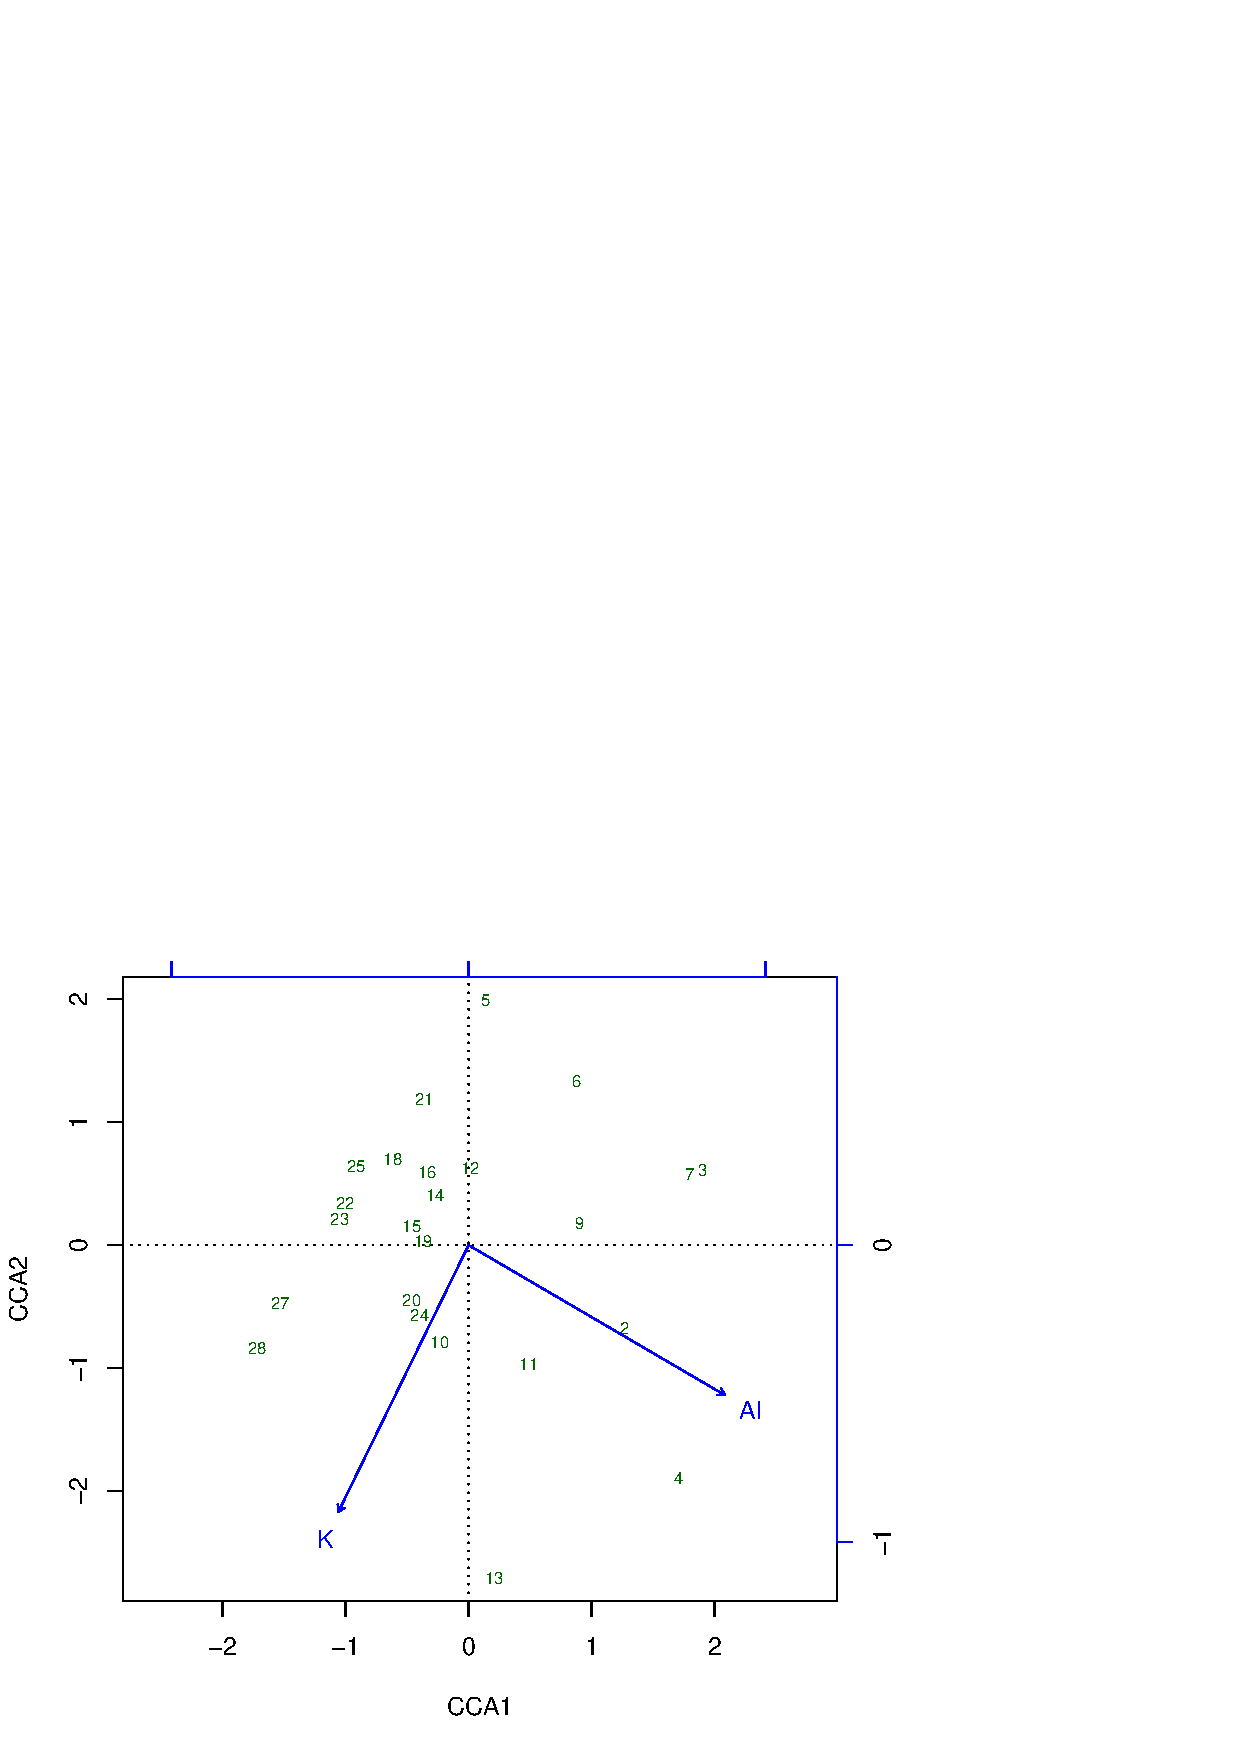
\includegraphics{vegan-FAQ-002}
\caption{LC scores in CCA of the original data.}
\label{fig:ccalc}
\end{center}
\end{figure}

What would happen to linear combinations of LC scores if we shuffle
the ordering of sites in species data?  Function \texttt{sample()} below
shuffles the indices.
\begin{Schunk}
\begin{Sinput}
> i <- sample(nrow(varespec))
> shuff <- cca(varespec[i, ] ~ Al + K, varechem)
\end{Sinput}
\end{Schunk}
\begin{figure}
\begin{center}
\begin{Schunk}
\begin{Sinput}
> plot(shuff, dis = c("lc", "bp"))
\end{Sinput}
\end{Schunk}
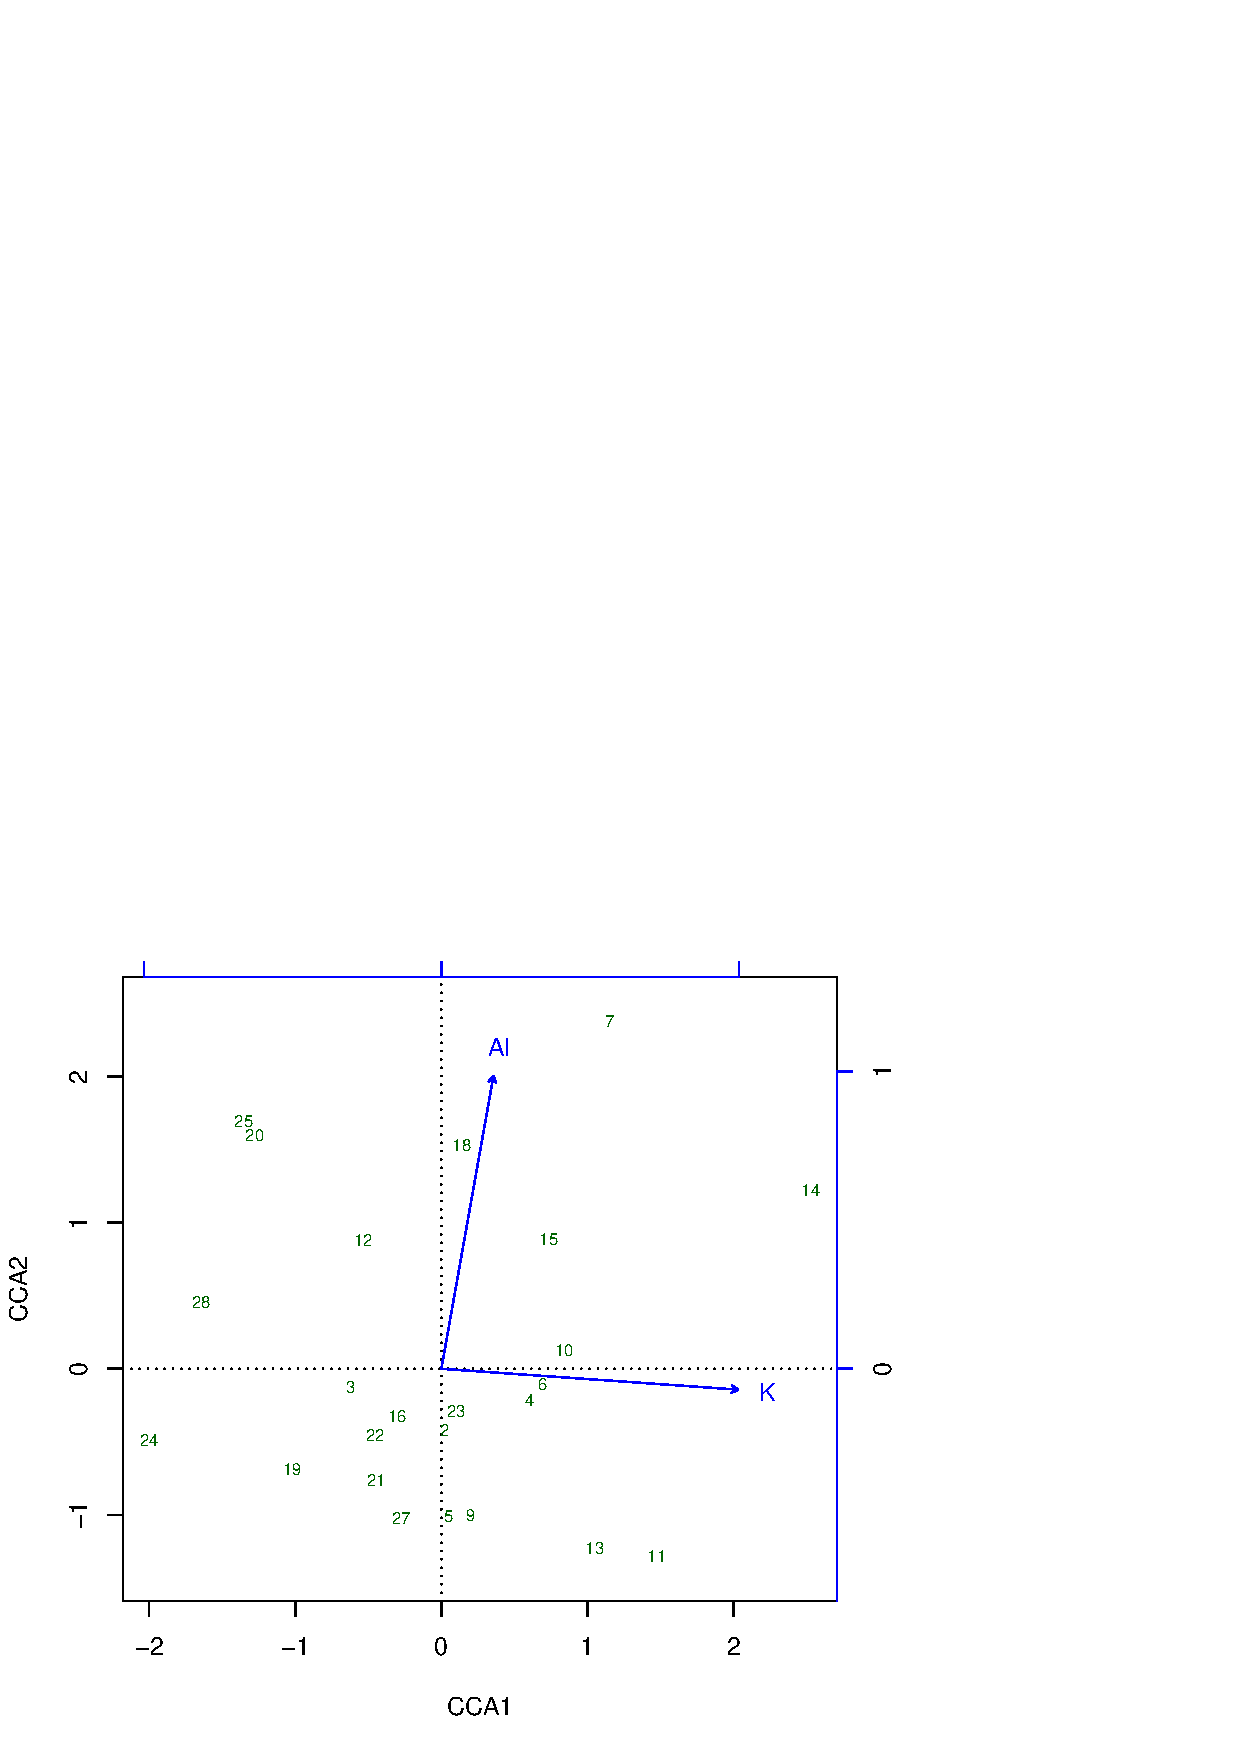
\includegraphics{vegan-FAQ-004}
\caption{LC scores of shuffled species data.}
\label{fig:ccashuff}
\end{center}
\end{figure}
It seems that site scores are fairly similar, but oriented differently
(Fig. \ref{fig:ccashuff}).  We can use Procrustes rotation to see how
similar the site scores indeed are (Fig. \ref{fig:ccaproc}).
\begin{figure}
\begin{center}
\begin{Schunk}
\begin{Sinput}
> plot(procrustes(scores(orig, dis = "lc"), scores(shuff, dis = "lc")))
\end{Sinput}
\end{Schunk}
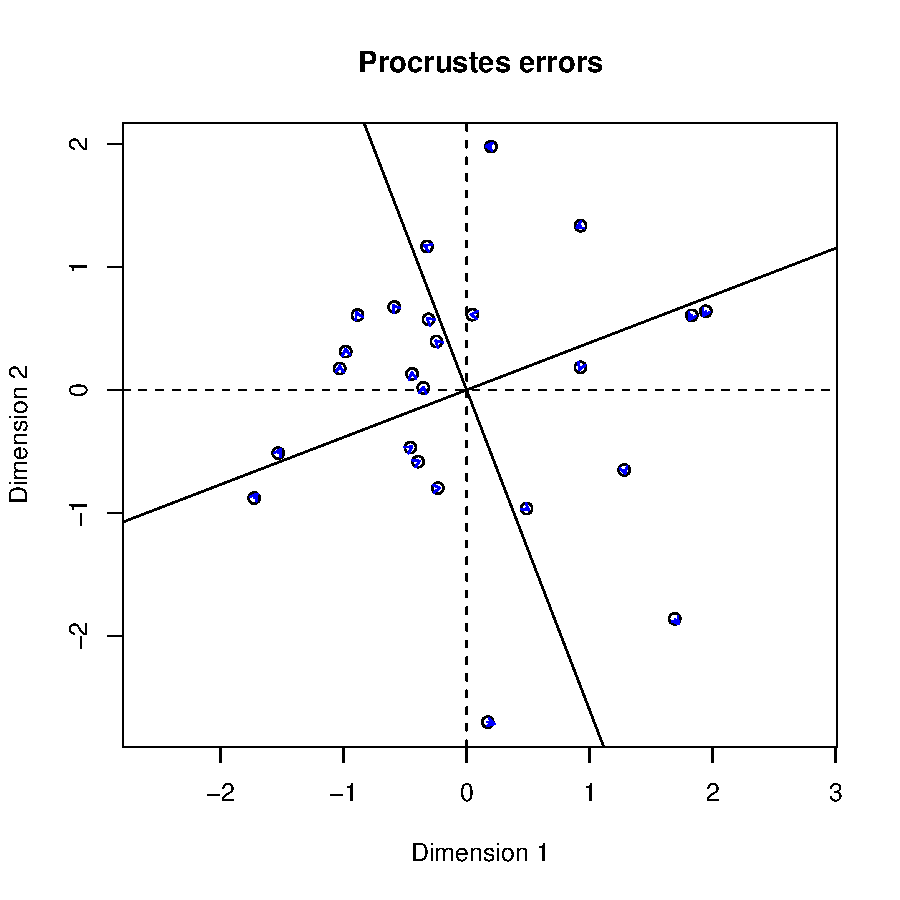
\includegraphics{vegan-FAQ-005}
\caption{Procrustes rotation of LC scores from CCA of original and shuffled data.}
\label{fig:ccaproc}
\end{center}
\end{figure}
There is a small difference, but this will disappear if we use
Redundancy Analysis (RDA) instead of CCA
(Fig. \ref{fig:rdaproc}). Here we use a new shuffling as well.
\begin{Schunk}
\begin{Sinput}
> tmp1 <- rda(varespec ~ Al + K, varechem)
> i <- sample(nrow(varespec))
> tmp2 <- rda(varespec[i, ] ~ Al + K, varechem)
\end{Sinput}
\end{Schunk}
\begin{figure}
\begin{center}
\begin{Schunk}
\begin{Sinput}
> plot(procrustes(scores(tmp1, dis = "lc"), scores(tmp2, dis = "lc")))
\end{Sinput}
\end{Schunk}
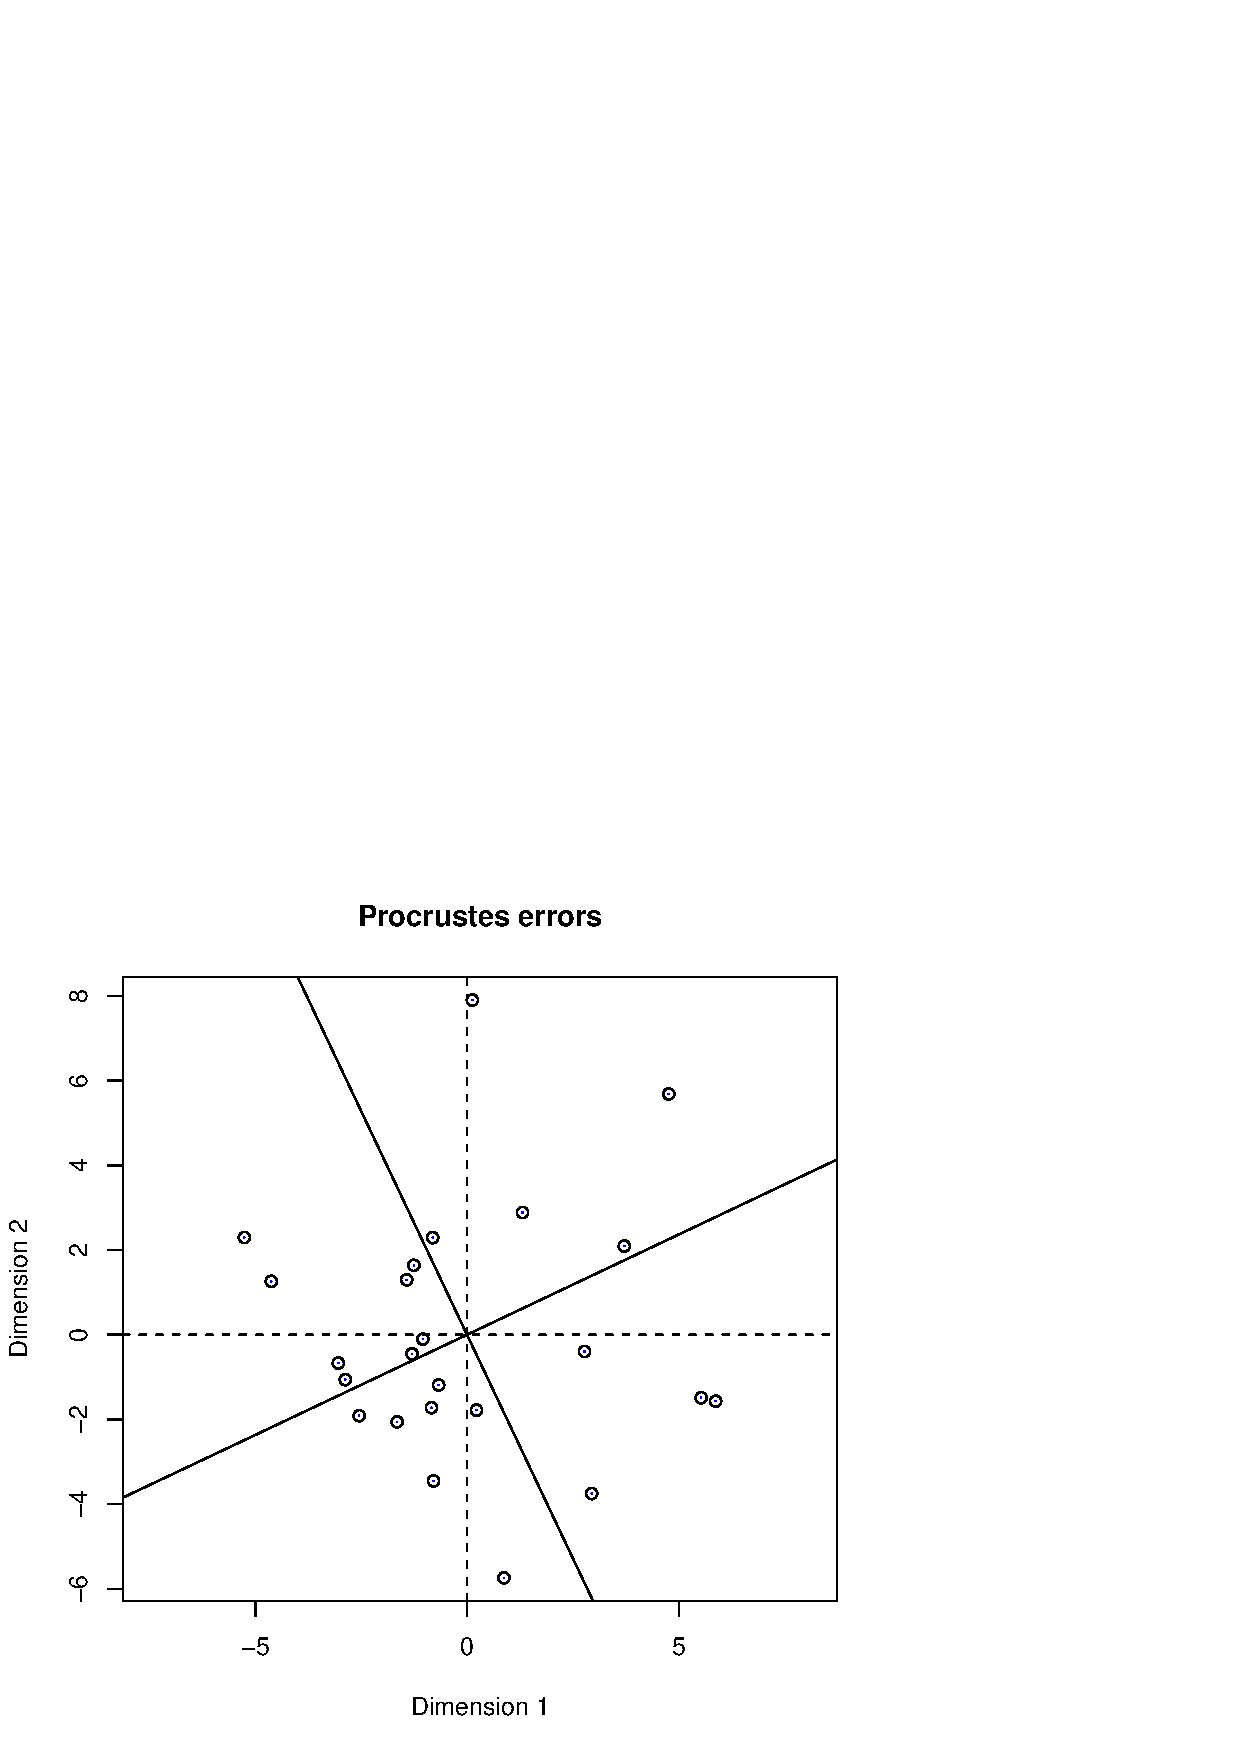
\includegraphics{vegan-FAQ-007}
\caption{Procrustes rotation of LC scores in RDA of the original and shuffled data.}
\label{fig:rdaproc}
\end{center}
\end{figure}

LC scores indeed are linear combinations of constraints (environmental
variables) and \emph{independent of species data}: You can
shuffle your species data, or change the data completely, but the LC
scores will be unchanged in RDA.  In CCA the LC scores are
\emph{weighted} linear combinations with site totals of species data
as weights. Shuffling species data in CCA changes the weights, and
this can cause changes in LC scores.  The magnitude of changes depends
on the variability of site totals.

The original data and shuffled data differ in their goodness of
fit\footnote{Or probably differ: The randomization is done while
generating this article, and different versions may have different
randomizations.}.
\begin{Schunk}
\begin{Sinput}
> orig
\end{Sinput}
\begin{Soutput}
Call:
cca(formula = varespec ~ Al + K, data = varechem) 

              Inertia Rank
Total           2.083     
Constrained     0.476    2
Unconstrained   1.607   21
Inertia is mean squared contingency coefficient 

Eigenvalues for constrained axes:
  CCA1   CCA2 
0.3608 0.1152 

Eigenvalues for unconstrained axes:
    CA1     CA2     CA3     CA4     CA5     CA6     CA7     CA8 
0.37476 0.24036 0.19696 0.17818 0.15209 0.11840 0.08364 0.07567 
(Showed only 8 of all 21 unconstrained eigenvalues)
\end{Soutput}
\begin{Sinput}
> shuff
\end{Sinput}
\begin{Soutput}
Call:
cca(formula = varespec[i, ] ~ Al + K, data = varechem) 

              Inertia Rank
Total          2.0832     
Constrained    0.2577    2
Unconstrained  1.8255   21
Inertia is mean squared contingency coefficient 

Eigenvalues for constrained axes:
   CCA1    CCA2 
0.21314 0.04453 

Eigenvalues for unconstrained axes:
    CA1     CA2     CA3     CA4     CA5     CA6     CA7     CA8 
0.39895 0.34101 0.22473 0.17163 0.15158 0.11558 0.10092 0.08716 
(Showed only 8 of all 21 unconstrained eigenvalues)
\end{Soutput}
\end{Schunk}
Similarly their WA scores will be (probably) very different
(Fig. \ref{fig:ccawa}).
\begin{figure}
\begin{center}
\begin{Schunk}
\begin{Sinput}
> plot(procrustes(orig, shuff))
\end{Sinput}
\end{Schunk}
\includegraphics{vegan-FAQ-009}
\caption{Procrustes rotation of WA scores of CCA with the original and
  shuffled data.}
\label{fig:ccawa}
\end{center}
\end{figure}

The example used only two environmental variables so that we can
easily plot all constrained axes.  With a larger number of
environmental variables the full configuration remains similarly
unchanged, but its orientation may change, so that two-dimensional
projections look different.  In the full space, the differences should
remain within numerical precision:
\begin{Schunk}
\begin{Sinput}
> tmp1 <- rda(varespec ~ ., varechem)
> tmp2 <- rda(varespec[i, ] ~ ., varechem)
> tmp1
\end{Sinput}
\begin{Soutput}
Call:
rda(formula = varespec ~ N + P + K + Ca + Mg + S + Al + Fe +      Mn + Zn + Mo + Baresoil + Humdepth + pH, data = varechem) 

              Inertia Rank
Total          1825.7     
Constrained    1459.9   14
Unconstrained   365.8    9
Inertia is variance 

Eigenvalues for constrained axes:
    RDA1     RDA2     RDA3     RDA4     RDA5     RDA6     RDA7     RDA8 
820.1042 399.2847 102.5617  47.6317  26.8382  24.0481  19.0644  10.1670 
    RDA9    RDA10    RDA11    RDA12    RDA13    RDA14 
  4.4288   2.2720   1.5353   0.9255   0.7155   0.3119 

Eigenvalues for unconstrained axes:
    PC1     PC2     PC3     PC4     PC5     PC6     PC7     PC8     PC9 
186.192  88.464  38.188  18.402  12.839  10.552   5.519   4.521   1.092 
\end{Soutput}
\begin{Sinput}
> proc <- procrustes(scores(tmp1, dis = "lc", choi = 1:14), scores(tmp2, 
+     dis = "lc", choi = 1:14))
> max(residuals(proc))
\end{Sinput}
\begin{Soutput}
[1] 2.032483e-14
\end{Soutput}
\end{Schunk}
In \texttt{cca} the difference would be somewhat larger than now
observed 2.0325e-14 because site
weights used for environmental variables are shuffled with the species
data.

\subsection{Factor constraints}

It seems that users often get confused when they perform constrained
analysis using  only one factor (class variable) as constraint.  The
following example uses the classical dune meadow data \cite{Jongman87}:
\begin{Schunk}
\begin{Sinput}
> data(dune)
> data(dune.env)
> summary(dune.env)
\end{Sinput}
\begin{Soutput}
       A1         Moisture Management       Use    Manure
 Min.   : 2.800   1:7      BF:3       Hayfield:7   0:6   
 1st Qu.: 3.500   2:4      HF:5       Haypastu:8   1:3   
 Median : 4.200   4:2      NM:6       Pasture :5   2:4   
 Mean   : 4.850   5:7      SF:6                    3:4   
 3rd Qu.: 5.725                                    4:3   
 Max.   :11.500                                          
\end{Soutput}
\begin{Sinput}
> orig <- cca(dune ~ Moisture, dune.env)
> orig
\end{Sinput}
\begin{Soutput}
Call:
cca(formula = dune ~ Moisture, data = dune.env) 

              Inertia Rank
Total          2.1153     
Constrained    0.6283    3
Unconstrained  1.4870   16
Inertia is mean squared contingency coefficient 

Eigenvalues for constrained axes:
  CCA1   CCA2   CCA3 
0.4187 0.1330 0.0766 

Eigenvalues for unconstrained axes:
     CA1      CA2      CA3      CA4      CA5      CA6      CA7      CA8 
0.409782 0.225913 0.176062 0.123389 0.108171 0.090751 0.085878 0.060894 
     CA9     CA10     CA11     CA12     CA13     CA14     CA15     CA16 
0.056606 0.046688 0.041926 0.020103 0.014335 0.009917 0.008505 0.008033 
\end{Soutput}
\end{Schunk}
When the results are plotted using LC scores, sample plots fall only
in four alternative positions (Fig. \ref{fig:factorlc}).
\begin{figure}
\begin{center}
\begin{Schunk}
\begin{Sinput}
> plot(orig, dis = "lc")
\end{Sinput}
\end{Schunk}
\includegraphics{vegan-FAQ-012}
\caption{LC scores of the dune meadow data using only one factor as a
  constraint.}
\label{fig:factorlc}
\end{center}
\end{figure}
In the previous chapter we saw that this happens because LC scores
\emph{are} the environmental variables, and they can be distinct only
if the environmental variables are distinct.  However, normally the user
would like to see how well the environmental variables separate the
vegetation, or inversely, how we could use the vegetation to
discriminate the environmental conditions.  For this purpose we should
plot WA scores, or LC scores and WA scores together:  The LC scores
show where the site \emph{should} be, the WA scores shows where the
site \emph{is}.

Function \texttt{ordispider} adds line segments to connect each WA
score with the corresponding LC (Fig.  \ref{fig:walcspider}).
\begin{figure}
\begin{center}
\begin{Schunk}
\begin{Sinput}
> plot(orig, display = "wa", type = "points")
> ordispider(orig, col = "red")
> text(orig, dis = "cn", col = "blue")
\end{Sinput}
\end{Schunk}
\includegraphics{vegan-FAQ-013}
\caption{A ``spider plot'' connecting WA scores to corresponding LC
  scores. The shorter the web segments, the better the ordination.}
\label{fig:walcspider}
\end{center}
\end{figure}
This is the standard way of displaying results of discriminant
analysis, too.  Moisture classes \texttt{1} and \texttt{2} seem to be
overlapping, and cannot be completely separated by their
vegetation. Other classes are more distinct, but there seems to be a
clear arc effect or a ``horseshoe'' despite using CCA.

\subsection{Conclusion}

LC scores are only the (weighted and scaled) constraints and
independent of vegetation. If you plot them, you plot only your
environmental variables. WA scores are based on vegetation data but
are constrained to be as similar to the LC scores as only
possible. Therefore \texttt{vegan} calls LC scores as
\texttt{constraints} and WA scores as \texttt{site scores}, and uses
primarily WA scores in plotting.  However, the user makes the ultimate
choice, since both scores are available.


\bibliographystyle{plain}
\bibliography{vegan}

\end{document}
